\begin{frame}
\frametitle{Prym varieties}


\begin{itemize}
	\item Start with an étale double cover \alert{$\widetilde C \xrightarrow{\pi} C$}.
	\pause
	\item Apply the Jacobian functor $J(-)$ to get a morphism:
	\begin{align*}
	\Nm\colon J\Big(\widetilde C\Big) &\to J(C) \\[1ex]
	\OO_{\widetilde C}\Big(\widetilde D\Big) &\mapsto \OO_C\Big(\pi_\ast \widetilde D\Big).
	\end{align*}
	\vskip-3ex
	\pause

	\item Then:
	\alert{
	\[
	\Prym\Big(\widetilde C, C\Big) \defeq (\ker \Nm)_0.
	\]
	}
\end{itemize}

\end{frame}


\begin{frame}
\frametitle{First properties of Pryms}

\begin{itemize}
	\item Every double cover comes with an involution $\sigma \colon  \widetilde C \circlearrowleft$ exchanging sheets.
\end{itemize}


\begin{proposition}
\[
(\ker Nm)_0 = \im(1-\sigma).
\]
\end{proposition}
\begin{proof}["Proof"]
One way is okay. Suppose $D= \sum a_i P_i - \sum a_i \sigma{P_i}$ is in the image. Then
\[
\Nm(D) = \sum a_i P_i - \sum a_i P_i = 0.
\]
\end{proof}
\end{frame}

\begin{frame}
\frametitle{The induced polarization}

The induced polarization comes from \alert{$i^\ast \Theta$}, where $i\colon\mkern-2mu\Prym\mkern-2mu\Big(\widetilde C, \C\Big)\mkern-2mu \to J(C)$ is the inclusion.

\begin{theorem}
The induced polarization on $P$ is twice a principal polarization.
\end{theorem}
\pause
\begin{remark}
In the complex setting, polarizations correspond to Hermitian forms on $\C^n\mkern-3mu$. It is principal if the Hermitian form can be written as 
\[
\begin{pmatrix*}[r]
0 & I \\
-I &0
\end{pmatrix*}
\]
in the standard basis.
\end{remark}
\end{frame}

\begin{frame}
\frametitle{Set-up}

\begin{itemize}
	\item Recall the description of $J\Big(\widetilde C\Big)$ as $H^0\Big(\widetilde C, \omega_{\widetilde C}\Big)^{\mkern-7mu\ast}/H_1\Big(\widetilde C, \Z\Big)$.
	\item We can identify
	\alert{
	\[
	\Prym\Big(\widetilde C, C\Big) = \Big(H^0\Big(\widetilde C, \omega_{\widetilde C}\Big)^{\mkern-7mu\ast}\Big)^{\mkern-7mu-} / {H_1\Big(\widetilde C, \Z\Big)}^{\mkern-7mu-}\mkern-7mu,
	\]
	}
	where the $(-)^-$, denotes the $-1$-eigenspaces.
\end{itemize}



\end{frame}


    \setbeamertemplate{navigation symbols}{}
    \begin{frame}[plain]
        \begin{tikzpicture}[remember picture,overlay]
            \node[at=(current page.center)] {
                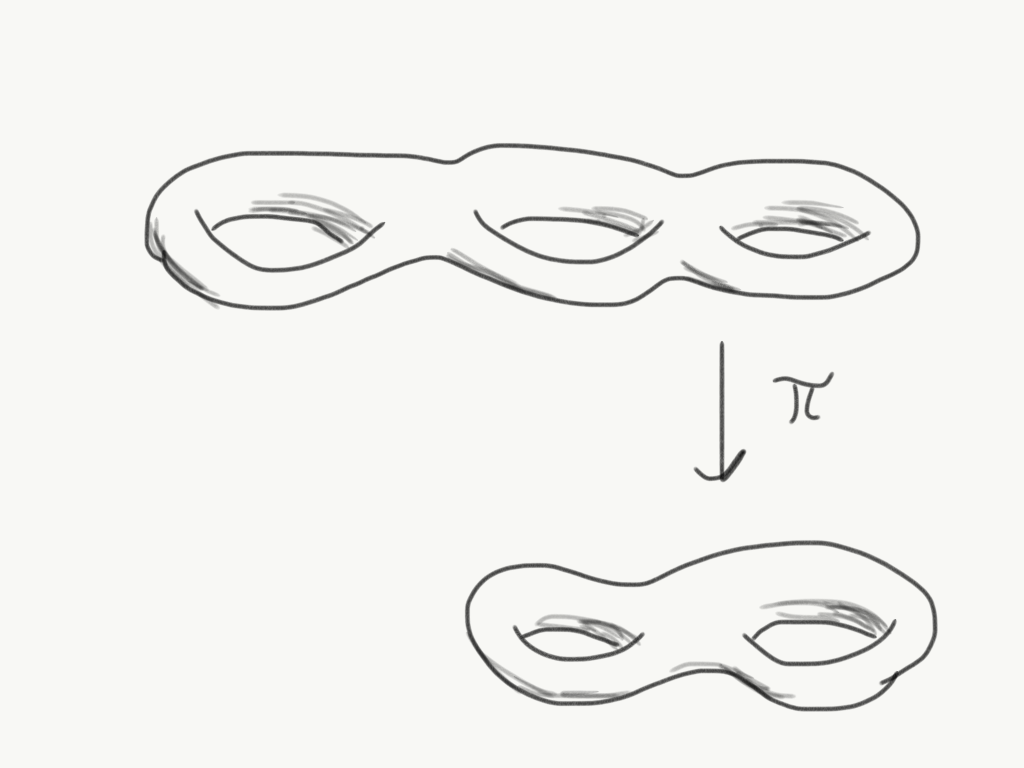
\includegraphics[width=\paperwidth]{sections/torus1}
            };
        \end{tikzpicture}
     \end{frame}

         \setbeamertemplate{navigation symbols}{}
    \begin{frame}[plain]
        \begin{tikzpicture}[remember picture,overlay]
            \node[at=(current page.center)] {
                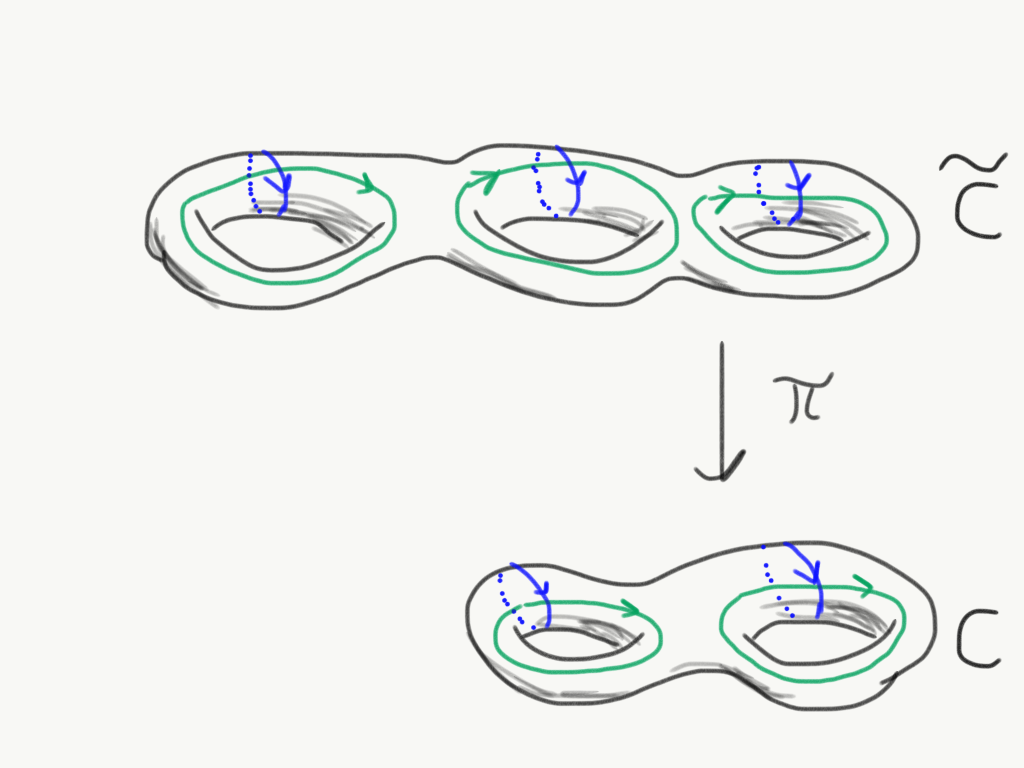
\includegraphics[width=\paperwidth]{sections/torus2}
            };
        \end{tikzpicture}
     \end{frame}


    \setbeamertemplate{navigation symbols}{}
    \begin{frame}[plain]
        \begin{tikzpicture}[remember picture,overlay]
            \node[at=(current page.center)] {
                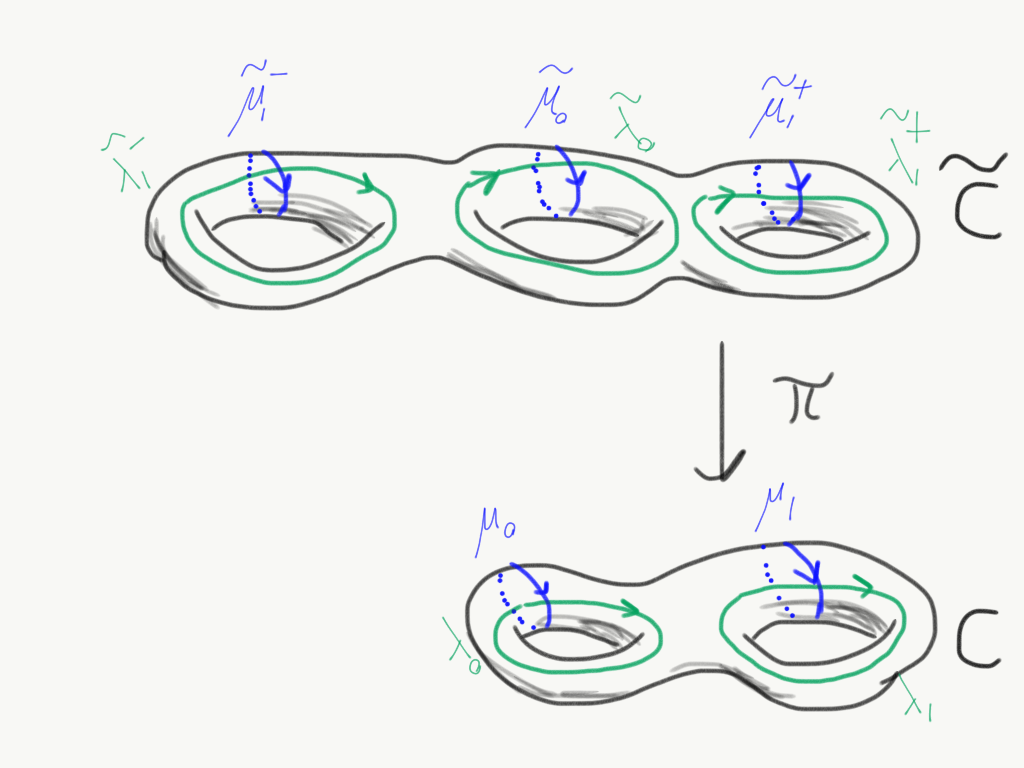
\includegraphics[width=\paperwidth]{sections/torus3}
            };
        \end{tikzpicture}
     \end{frame}


\begin{frame}
    

\begin{enumerate}[<+->]
	\item Choose a symplectic basis $\lambda_0, \ldots, \lambda_g$, $\mu_0, \ldots, \mu_g$ of $H_1(C,\Z)$.

	\item A degree $2$ covering is determined by a cycle $\mu_0$ in $H_1(C, \Z/2)$.

	\item A symplectic basis for $H_1\Big(\widetilde C, \Z\Big)$ consists of the lifts $\widetilde{\mu^+}_i, \widetilde{\mu^-}_i$, $\widetilde{\lambda^-}_i, \widetilde{\lambda^+}_i$ and $\widetilde{\mu}_0, \widetilde{\lambda}_0$. (From this we see that $\widetilde C$ has genus $2g+1$ if $C$ has genus $g-1$)

	\item A basis for the $(-1)$-eigenspace of $H_1(\widetilde C,\Z)$ is then
	\begin{align*}
	\alpha_i \defeq \lambda_i^+ - \lambda_i^-, && \beta_i \defeq \mu_i^+ - \mu_i^- && i=1,\ldots, g
	\end{align*}

	\item The restriction of the Hermitian form is:
	\begin{align*}
	E\big(\alpha_i,\beta_j\big)= 2 \delta_{ij} && E\big(\alpha_i, \alpha_j\big) = E\big(\beta_i,\beta_j\big)=0,
	\end{align*}
	which means it is twice a principal polarization.
\end{enumerate}


\end{frame}